\documentclass[12pt,english]{article}
\usepackage[a4paper,bindingoffset=0.2in,%
            left=1in,right=1in,top=1in,bottom=1in,%
            footskip=.25in]{geometry}
\usepackage{blindtext}
\usepackage{titling}
\usepackage{amssymb}
\usepackage{amsmath}
\usepackage{listings}
\usepackage{lettrine} 
\usepackage{tikz}  
\usepackage{color} 
\usepackage{verbatim}
\usepackage{pgfplots}
\usepgfplotslibrary{external}
\pgfplotsset{width=10cm,compat=1.9}
%================================
\begin{document}
\newgeometry{left=0.8in,right=0.8in,top=1in,bottom=1in}
\begin{center}
    \Large
    \textbf{Homework 7}\\
    \small
    \today\\
    \large
    Jose Carlos Munoz
\end{center}%===============================
Q6.a)\\
Q6.b)\\
Q6.c)\\
Q6.d)\\
Q6.e)\\
Q16)\par
The Following is for the Single Link\\
\begin{equation*}
\begin{array}{c|ccc}
\mbox{-}& \mbox{DT} & \mbox{GD} & \mbox{V}\\
\hline
\mbox{DT} & \left[ 0,0,23 \right]& \left[ 10,2,11\right]& \left[ 2,6,15 \right]\\
\mbox{GD} & \left[ 2,10,11\right]& \left[ 0,0,23 \right]& \left[ 0,8,15 \right]\\
\mbox{V}  & \left[ 6,2,15 \right]& \left[ 8,0,15 \right]& \left[ 0,0,23 \right]
\end{array}
\end{equation*}
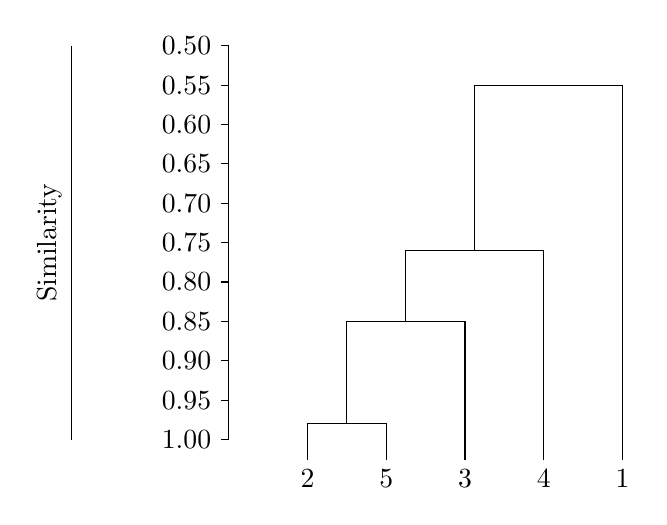
\begin{tikzpicture}[sloped]
    \node (a) at (-6,-0.5) {2};
    \node (b) at (-5,-0.5) {5};
    \node (c) at (-4,-0.5) {3};
    \node (d) at (-3,-0.5) {4};
    \node (e) at (-2,-0.5) {1};
    \node (ab) at (-5.5,0.2) {};
    \node (abc) at (-4.75,1.5){};
    \node (abcd) at (-3.875,2.4) {};
    \node (abcde) at (-2.9375,4.5) {};
    
    \draw  (a) |- (ab.center);
    \draw  (b) |- (ab.center);
    \draw  (c) |- (abc.center);
    \draw  (d) |- (abcd.center);
    \draw  (e) |- (abcde.center);
    \draw  (ab.center) |- (abc.center);
    \draw  (abc.center) |-(abcd.center);
    \draw  (abcd.center) |-(abcde.center);
 
    \draw[] (-9,0) -- node[above]{Similarity} (-9,5);
    \draw (-7,0) -- (-7,5);
    
    \foreach \y in {0,0.5,1,1.5,2,2.5,3,3.5,4,4.5,5}                     
    \draw[shift={(0,\y)},color=black] (-7,0) -- (-7.1,0);
    
    \node[left] at (-7.1,0.0) {$1.00$} ;
    \node[left] at (-7.1,0.5) {$0.95$} ;
    \node[left] at (-7.1,1.0) {$0.90$} ;
    \node[left] at (-7.1,1.5) {$0.85$} ;
    \node[left] at (-7.1,2.0) {$0.80$} ;
    \node[left] at (-7.1,2.5) {$0.75$} ;
    \node[left] at (-7.1,3.0) {$0.70$} ;
    \node[left] at (-7.1,3.5) {$0.65$} ;
    \node[left] at (-7.1,4.0) {$0.60$} ;
    \node[left] at (-7.1,4.5) {$0.55$} ;
    \node[left] at (-7.1,5.0) {$0.50$} ;
    
\end{tikzpicture}
\par
The Following is for the Complete Link\\
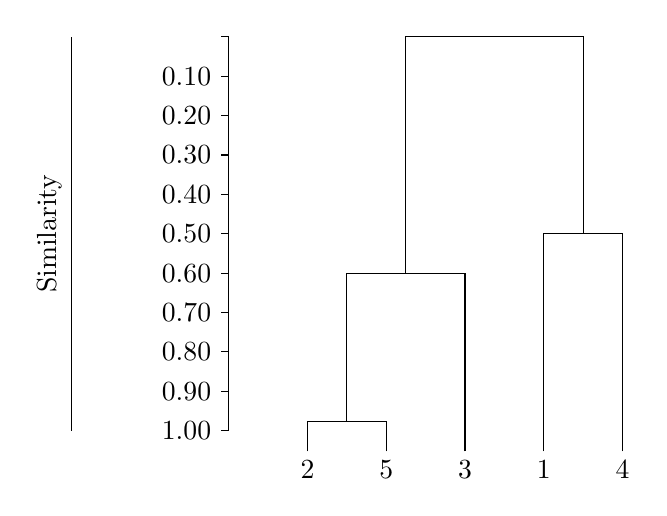
\begin{tikzpicture}[sloped]
    \node (a) at (-6,-0.5) {2};
    \node (b) at (-5,-0.5) {5};
    \node (c) at (-4,-0.5) {3};
    \node (d) at (-3,-0.5) {1};
    \node (e) at (-2,-0.5) {4};
    \node (ab) at (-5.5,0.11) {};
    \node (abc) at (-4.75,2){};
    \node (cd) at (-2.5,2.5) {};
    \node (abcde) at (-2.9375,5) {};
    
    \draw  (a) |- (ab.center);
    \draw  (b) |- (ab.center);
    \draw  (c) |- (abc.center);
    \draw  (d) |- (cd.center);
    \draw  (e) |- (cd.center);
    \draw  (ab.center) |- (abc.center);
    \draw  (abc.center) |-(abcde.center);
    \draw  (cd.center) |-(abcde.center);
 
    \draw[] (-9,0) -- node[above]{Similarity} (-9,5);
    \draw (-7,0) -- (-7,5);
    
    \foreach \y in {0,0.5,1,1.5,2,2.5,3,3.5,4,4.5,5}                     
    \draw[shift={(0,\y)},color=black] (-7,0) -- (-7.1,0);
    
    \node[left] at (-7.1,0.0) {$1.00$} ;
    \node[left] at (-7.1,0.5) {$0.90$} ;
    \node[left] at (-7.1,1.0) {$0.80$} ;
    \node[left] at (-7.1,1.5) {$0.70$} ;
    \node[left] at (-7.1,2.0) {$0.60$} ;
    \node[left] at (-7.1,2.5) {$0.50$} ;
    \node[left] at (-7.1,3.0) {$0.40$} ;
    \node[left] at (-7.1,3.5) {$0.30$} ;
    \node[left] at (-7.1,4.0) {$0.20$} ;
    \node[left] at (-7.1,4.5) {$0.10$} ;
    
\end{tikzpicture}
\par
Q17.a)\\
Q17.b)\\
Q17.c)\\
Q17.d)\\
Q17.e)\\
Q17.f)\\
\end{document}
